\documentclass{litesolution}
\usepackage[level]{datetime}

\makeatletter
\definecolor{pkgcolor}{Hsb}{103,.8,.5}
\definecolor{moducolor}{Hsb}{290,.8,.5}
\definecolor{cmdcolor}{Hsb}{188,.8,.5}
\definecolor{filecolor}{Hsb}{207,.6,.7}
\definecolor{H1}{Hsb}{349,.8,.8}% 海棠紅 (Hangzhou MTR L 1 )
\definecolor{H2}{Hsb}{23, .8,.8}% 丹桂橙 (Hangzhou Metro 2 )
\definecolor{H3}{Hsb}{48, .8,.8}% 柠檬黄 (Hangzhou Metro 3 )
\definecolor{H4}{Hsb}{103,.8,.8}% 香樟绿 (Hangzhou Metro 4 )
\definecolor{H5}{Hsb}{188,.8,.8}% 青藍色 (Hangzhou MTR L 5 )
\definecolor{H6}{Hsb}{207,.8,.8}% 海洋蓝 (Hangzhou Metro 6 )
\definecolor{H7}{Hsb}{290,.8,.8}% 浪漫紫 (Hangzhou Metro 7 )
\hypersetup{colorlinks,urlcolor=H1,linkcolor=H2,filecolor=filecolor,pdfstartview=FitH,pdfview=FitH,pdfcreator=XeTeX output}

\def\@pkg#1{\texorpdfstring{\href{https://www.ctan.org/pkg/#1}{\textcolor{pkgcolor}{\textsf{#1}}}}{“#1”}}
\def\s@pkg#1{\texorpdfstring{\textcolor{pkgcolor}{\textsf{#1}}}{“#1”}}
\DeclareRobustCommand\pkg{\@ifstar\s@pkg\@pkg}
\def\mode#1{\texorpdfstring{\textcolor{moducolor}{\textsf{#1}}}{“#1”}}
\def\cmd#1{\texorpdfstring{\textcolor{cmdcolor}{\textsf{#1}}}{“#1”}}
\def\datechange#1#2{%
  \noindent{\makebox[\textwidth][r]{\color{H7}\rule{1.15\textwidth}{.4pt}}}
  \noindent\makebox[0pt][r]{\makebox[-3em][r]{\small\textbf{\textcolor{H7}{#1}}}\;\;}{\sffamily Update: \ignorespaces#2}}
\makeatother

% \watermark{ctanlion}

\begin{document}

\chapterimage{cover1.png}
\chapter{The \pkg{LiteSolution} Template}
\fancyhead[L]{\,\color{H7}\href{https://github.com/xiamyphys/litesolution}{\faIcon{github}\;\leftmark}}
\fancyhead[R]{\color{H7}\rightmark\,}

\centerline{Xia Mingyu, \href{https://www.hdu.edu.cn}{Hangzhou Dianzi University}}
\ddmmyyyydate
\centerline{\mailto{xiamyphys@gmail.com}}
\centerline{\today,\quad Version 1.0a}

This is the document for \pkg{LiteSolution} template, which provides a lite design of the solution of test paper.

Some designs of this template currently only support \textbf{Simplified Chinese (Mainland)}. If necessary, you can change some Chinese characters to the language you want in the \verb|*.cls| file.

\section{Introduction}
\subsection{The purpose of this template}
This template provides a lite and fresh template, and mainly used for typesetting solutions of final, textbooks' and other exercises. This template is developed based on \pkg{ElegantBook} and \href{https://github.com/Azure1210/VividBooK}{\pkg*{VividBooK}}, ported and improved the chapter design module code of \href{https://www.overleaf.com/latex/templates/the-legrand-orange-book-template-english/jtctyfmnpppc}{\pkg*{The Legrand Orange Book}}. I'd like to express my gratitude to the template authors above for their previous work.

If you meet bugs when using this template, or you have better suggestions or ideas, or you want to participate in the development of the template or other templates by me, welcome to contact via email \href{mailto:xiamyphys@gmail.com}{xiamyphys@gmail.com}.

Also, you can join my \textsf\LaTeX{} Template Discussion \href{https://qm.qq.com/q/OnHzbNvVAG}{QQ Group: 760570712} to communicate with me and get the insider preview edition of the template.

\subsection{Loading \pkg{LiteSolution} and its modes}

You should update all the packages to the latest version or switch to portable version instead by implementing the commands 
\begin{verbatim}
    tlmgr update --self
    tlmgr update --all
    tlmgr update --self --all --reinstall-forcibly-removed
\end{verbatim}

To learn more, please refer to \href{https://tex.stackexchange.com/questions/55437/how-do-i-update-my-tex-distribution}{How do I update my TEX distribution?}

Save the file \verb|litesolution.cls| to your project's root directory, and then create a \verb|.tex| file, just input the command \verb|\documentclass{litesolution}| on the first line.

The template provides 3 modes, \mode{answer}, \mode{mtpro2} and \mode{counter}. Just add the options of the modes you want separately in the square bracket of the command \verb|\documentclass[options]{litesolution}| in your \verb|.tex| file.

\section{Modes of \pkg{LiteSolution}}
\subsection{The \mode{answer} mode}
This mode has two options, \mode{ans} and \mode{noans}, which can show and hide answers respectively. After you choose the \mode{noans}, the contents in the environment \cmd{solution}, the command \cmd{ans} and the answers in the multiple choice questions will all become the same color as the pagecolor. So the area that originally contained the answer will be replaced by an area of the same blank size. You can generate exams without answers and solutions by enabling \mode{noans}.

\subsection{The \mode{mtpro2} mode}
If you've installed the \emph{Mathtime Pro 2 Lite} font in your computer, then you can use this mode to change the math font.

\subsection{The \mode{counter}}
This mode has two options, \mode{separate} and \mode{continuous}, which can make the page counter between chapters be remaked or continuous.The page numbers between each test question will be continuous when you use the \mode{continuous} mode or the page number of each test question will start from 1 when you use the \mode{separate}.


\section{Commands of \pkg{LiteSolution}}
\subsection{The \cmd{chapterimage} command}
\begin{verbatim}
    \chapterimage{cover1.png}
\end{verbatim}
This command can assign the title background image for each subsequent chapter.

\subsection{The \cmd{chapterfont} command}
This command can assign the title font for each subsequent chapter, if you do not use this command, the title font will be \emph{songti} in Chinese and \emph{Libertinus} in English.

\subsection{The \cmd{ans} command}
This command can underlines the answer and changes the color of the answer to \textcolor{1号色}{Blue Sapphire}.

\paragraph{If mode \mode{noans} is enabled, the answer will disappear, leaving only a horizontal line the same width as the answer.}

\subsection{The \cmd{watermark} command}
\begin{verbatim}
    \watermark{ctanlion.pdf}
\end{verbatim}

This command can add watermark to the document.

\subsection{Other customer commands}
In order to facilitate input, the following commands are scheduled. You can add others in the \verb|*.cls| file as you like.
\vskip1em
\begin{center}
    \begin{tabular}{l|l|l|l|l|l}
        \toprule
        Command & Output & Command & Output & Command & Output\\
        \midrule
        \verb|\titlelogo{#1}{#2}| & Add emoji with link in text & \verb|\point{#1}| & Add score & \verb|\i| & $\mathrm{i}$\\
        \hline
        \verb|\sokka{#1}| & 故本题选择\#1项 & \verb|\d| & $\mathrm{d}$ & \verb|\e| & $\mathrm{e}$\\
        \bottomrule
    \end{tabular}    
\end{center}

\section{Environments of \pkg{LiteSolution}}
\subsection{The \cmd{choice} environment}
There're two variables in this envrionment. The first one is the answer of the choice problem, the second one is the keywords of this choice problem and it's optional.

\begin{tcblisting}{sidebyside}
\begin{choice}{D}[Keywords]
If you want to add choice and keywords.
\begin{tasks}(2) % 2 choices per line
    \task This is choice A  \task This is choice B
    \task This is choice C  \task This is choice D
\end{tasks}
\end{choice}
\begin{choice}{D}
If you want to add choice only.
\begin{tasks}(4) % 4 choices per line
    \task Chc A \task Chc B \task Chc C \task Chc D
\end{tasks}
\end{choice}
\end{tcblisting}

\begin{paracol}{2}
    \begin{choice}{D}[Gaussian theory]
        $A$和$B$为两个均匀带电球体,$A$带电荷$+q$,$B$带电荷$-q$,作一与$A$...
        \begin{tasks}(2)
            \task 通过$S$面的电场强度...        \task 通过$S$面的电场强度...
            \task 通过$S$面的电场强度...        \task 通过$S$面的电场强度...
        \end{tasks}
    \end{choice}
    \switchcolumn
    \centering\vfill
    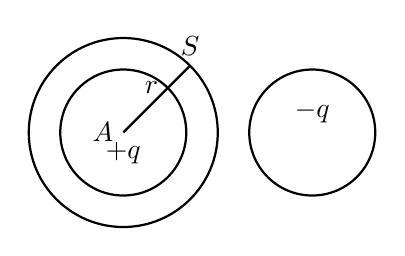
\begin{tikzpicture}
        \draw [thick] (0,0) circle (0.8);
        \draw [thick] (0,0) circle (1.2);
        \draw [thick] (2.4,0) circle (0.8);
        \draw [thick] (0,0)--(0.85,0.85);
        \node [anchor=east] at (0,0) {$A$};
        \node [anchor=north] at (0,0) {$+q$};
        \node [anchor=east] at (0.566,0.566) {$r$};
        \node [anchor=south] at (0.85,0.85) {$S$};
        \node [anchor=south] at (2.4,0) {$-q$};
    \end{tikzpicture}
    \vfill
\end{paracol}
\begin{verbatim}
\begin{paracol}{2}
\begin{choice}{D}[Gaussian theory]
    $A$和$B$为两个均匀带电球体,$A$带电荷$+q$,$B$带电荷$-q$,作一与$A$...
    \begin{tasks}(2)
        \task 通过$S$面的电场强度...        \task 通过$S$面的电场强度...
        \task 通过$S$面的电场强度...        \task 通过$S$面的电场强度...
    \end{tasks}
\end{choice}
\switchcolumn\centering\vfill\tikz{...}\vfill
\end{paracol}
\end{verbatim}

\subsection{The \cmd{problem} environment}
Sightly different from the cmd{choice} environment: the two variables are points and keywords, and the question number counter is shared with the multiple-choice question number counter.
\begin{tcblisting}{sidebyside}
    \begin{problem}[Keywords][5]
        If you want to add keywords and points.
    \end{problem}
    \begin{problem}
        If you want to add none.
    \end{problem}
    \begin{problem}[Keywords]
        If you want to add keywords only.
    \end{problem}
    \begin{problem}*[][5]
        If you want to add points only.
    \end{problem}
\end{tcblisting}

\begin{paracol}{2}
\begin{problem}[Gaussian theory \& Field strength][6]
    一均匀带电直导线长为$d$,电荷线密度为$+\lambda$.过导线中点$O$作一半径为$R$($R>\frac{d}{2}$)的球面$S$,$P$为带电直导线的延长线与球面$S$的交点. 则通过该球面的电场强度通量$\Phi_e=$\ans{$\frac{\lambda d}{\varepsilon_0}$},带电直线的延长线与球面交点$P$处的电场强度的大小为\ans{$\frac{\lambda d}{4\pi\varepsilon_0(R^2-d^2/4)}$},方向\ans{沿矢径$\boldsymbol{OP}$}.
    \end{problem}
\switchcolumn\centering
\vfill
\begin{tikzpicture}[scale=0.83]
    \draw (0,0) circle (2);
    \draw [thick,->] (-2,0)--(0,0)--(1,1.732);
    \node [anchor=east] at (-2,0) {$P$};
    \filldraw (-2,0) circle (0.05);
    \node [anchor=west] at (0.5,0.866) {$R$};
    \filldraw [pattern=north east lines] (-0.8,-0.1)--(-0.8,0.1)--(0.8,0.1)--(0.8,-0.1)--cycle;
    \draw [thick,|<-] (-0.8,-0.3)--(-0.25,-0.3);
    \draw [thick,|<-] (0.8,-0.3)--(0.25,-0.3);
    \node at (0,-0.3) {$L$};
\end{tikzpicture}
\vfill
\end{paracol}
\begin{verbatim}
\begin{paracol}{2}
    \begin{problem}[Gaussian theory \& Field strength][6]
        一均匀带电直导线长为$d$,电荷线密度为$+\lambda$,过导线中点$O$...
        场强大小\ans{$\frac{\lambda d}{4\pi\varepsilon_0(R^2-d^2/4)}$}...
    \end{problem}
\switchcolumn\centering\vfill\tikz{...}\vfill
\end{paracol}
\end{verbatim}

\subsection{The \cmd{note} environment}
\begin{tcblisting}{sidebyside}
\begin{note}
    Please note that...
\end{note}
\end{tcblisting}

\subsection{The \cmd{solution} environment}
\begin{tcblisting}{sidebyside}
\begin{solution}
    This is the answer for the problem.
\end{solution}
\end{tcblisting}

If a star (*) is added after the \verb|\begin{solution}|, then the content will follow the 
\begin{tcblisting}{sidebyside}
\begin{solution}*
    This is the answer for the problem.
\end{solution}
\end{tcblisting}

\paragraph{If mode \mode{noans} is enabled, the solution will disappear, leaving only a blank box with the same height as the solution, and the name of the box will change to \emph{\textcolor{1号色}{\textbf{\faIcon{ban} 答案隐藏}}}.}

\newpage
\section{Version History}
This template is used to type the mid-term and final exam solutions of \emph{College Physics}. Initially, I used the \href{https://www.ctan.org/pkg/elegantbook}{ElegantBook} template for layout, however, it's no longer be maintained since January 1st, 2023, so I trun to use the \href{https://github.com/Azure1210/VividBooK}{\pkg*{VividBooK}} instead. But this template is too bloated and some functions \& designs need to be redesigned, so I started developing \pkg{LiteSolution}.

\textsf{\bfseries Version 0.1a} was finished developing on 29 June, 2023 and released on \href{https://mp.weixin.qq.com/s/kd4StYk3XybhNQZkAfoY6A}{\faIcon{weixin} WeChat Public Account: 物理问题作} with the name \emph{FreshSolution}. This version redesigned the \cmd{exercise} environment and the \cmd{solution} environment in terms of designs and functions, and improvements have been made to the design of the chapterimage part.

\textsf{\bfseries Version 0.1b} was finished developing on 6 July, 2023 and released on \href{https://www.latexstudio.net/index/details/index/mid/3553.html}{LaTeX Studio} (Xiaoshan, Hangzhou) and \href{http://xhslink.com/YBuuuw}{Xiaohongshu}, where won the favor of many people. This version has added the global option to make the page number be remaked or continuous between chapters, and command \cmd{watermark} has been added in this version.

\textsf{\bfseries Version 1.0a} was finished developing on 15 November, 2023. This version has redesigned the \cmd{chapterimage} part, \cmd{choice} and replaced the \cmd{exercise} environment with the \cmd{problem} environment.

\datechange{06/07/2023}{Version 0.1b}
\begin{itemize}
    \item Support page number remaking between chapters.
    \item Added \cmd{watermark} command.
\end{itemize}

\datechange{15/11/2023}{Version 1.0a}
\begin{itemize}
    \item Redesigned the \cmd{chapterimage} part, include the layout and the code.
    \item Redesigned the \cmd{choice} and \cmd{solution} environment, keywords become optional and supports star (*) key. 
    \item Replaced the \cmd{exercise} environment with the \cmd{problem} environment, supports adding only keywords or points.
    \item Added the \cmd{note} environment and some customer commands.
\end{itemize}

\subsection*{Future Plans}
\begin{itemize}
    \item Plan to integrate the color management of \href{https://www.ctan.org/pkg/elegantbook}{\pkg*{ElegantBook}}.
    \item Plan to integrate the chapter design of \href{https://www.ctan.org/pkg/elegantbook}{\pkg*{ElegantBook}} into the star (*) key value of this template \cmd{chapter}.
    \item Plan to add the \mode{dark} mode to this template to make the text color light while make the page color dark to protect eyesight.
    \item Plan to change the \verb|*.cls| file to a block code design to make it easier for subsequent developers to maintain or modify.
    \item ......
\end{itemize}
\chapter{A Sample for \pkg{LiteSolution} Template}
\fancyhead[L]{\color{H6}\kaishu\faIcon{atom}\;2023年\titlelogo{https://sci.hdu.edu.cn}{HDU}「大学物理2」期中模拟}
\fancyhead[R]{\color{H6}\kaishu\rightmark\,}

\date{2023年12月3日}{大学物理教学团队}{A0715012}
{\href{https://qm.qq.com/q/UPbGudx8cK}{\textbf{物理問題作}}}
{https://qm.qq.com/q/asJiytD5pC}{HDU 物理营}
{http://weixin.qq.com/r/mhKYgFTEMQlOrRDj90eI}{未央学社公众号}

\section{选择题(每题3分,共36分)}
\begin{choice}{D}[弹簧振子]
    一劲度系数为$k$的轻弹簧,下端挂一质量为$m$的物体,系统的振动周期为$T_1$. 若将此弹簧截去一半的长度,下端挂一质量为$m/2$的物体,则系统振动周期$T_2$等于
\begin{tasks}(4)
    \task $2T_1$
    \task $T_1$
    \task $\frac{T_1}{\sqrt2}$
    \task $\frac{T_1}{2}$
\end{tasks}
\end{choice}
\begin{solution}*
    弹簧的劲度系数与长度成反比,所以剪断一半后劲度系数变为$2k$;根据弹簧振子的周期表达式$T=2\pi\sqrt{\frac mk}$可知此时的周期$T_2=2\pi\sqrt{\frac{m/2}{2k}}=\frac{T_1}{2}$.\sokka{D}
\end{solution}

\begin{choice}{B}[单摆]
    把单摆摆球从平衡位置向位移正方向拉开,使摆线与竖直方向成一微小角度$\theta$,然后由静止放手任其振动,从放手时开始计时.若用余弦函数表示其运动方程,则该单摆振动的初相为
    \begin{tasks}(4)
        \task $\theta$
        \task $0$
        \task $\frac\pi2$
        \task $-\pi$
    \end{tasks}
\end{choice}

\vskip-2ex
\begin{paracol}{2}
\begin{choice}{A}[平面简谐波的波函数]
    一平面简谐波,波速$u=5\mathrm{m/s}$,$t=3\mathrm{s}$时波形曲线如图,则$x=0$处质点的振动方程可能为
\begin{tasks}(2)
    \task $y=2\ee{-2}\cos\ab(\frac12\pi t-\frac12\pi)$
    \task $y=2\ee{-2}\cos\ab(\frac12\pi t+\frac12\pi)$
    \task $y=2\ee{-2}\cos(\pi t+\pi)$
    \task $y=2\ee{-2}\cos\ab(\pi t-\frac32\pi)$
\end{tasks}
\end{choice}
\switchcolumn\centering
\vfill
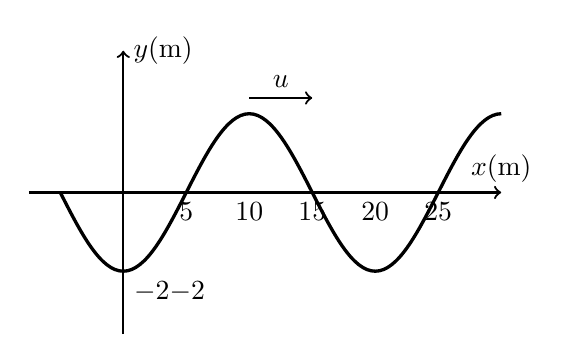
\begin{tikzpicture}
    \draw [->,thick] (-1.2,0) -- (4.8,0) node [anchor=south] {$x(\mathrm{m})$};
    \draw [->,thick] (0,-1.8) -- (0,1.8) node [anchor=west] {$y(\mathrm{m})$};
    \draw [very thick] (-.8,0) sin (0,-1) node [anchor=north west] {$-2\ee{-2}$} cos (.8,0) sin (1.6,1) cos (2.4,0) sin (3.2,-1) cos (4,0) sin (4.8,1);
    \draw [thick,->] (1.6,1.2) -- (2.4,1.2) node [midway,anchor=south] {$u$};
    \foreach \a in {5,10,...,25}
    \node [anchor=north,xshift=0.16*\a cm] at (0,0) {\a};
\end{tikzpicture}
\vfill
\end{paracol}
\vspace{-.75em}
\begin{solution}*
    由图可知$A=0.02\mathrm{m},\ \omega=\frac{2\pi u}{\lambda}=\frac12\pi$.由于原点处$v>0$,所以初相$\varphi=-\frac\pi2$.\sokka{A}
\end{solution}

\begin{choice}{A}[增透膜]
    一艘油船行经我国台湾岛东部海域时发生石油泄漏,在海面上形成大片油膜,太阳光在头顶正射时,救授人员乘直升飞机从上往下看,发现油膜对$552\mathrm{nm}$波长的可见光反射形成干涉相长而最亮,则可以推测该区域油膜厚度可能为多少?(设石油折射率$n=1.2$,海水折射率$n=1.3$)
\begin{tasks}(4)
    \task $460\mathrm{nm}$
    \task $552\mathrm{nm}$
    \task $345\mathrm{nm}$
    \task $425\mathrm{nm}$
\end{tasks}
\end{choice}
\begin{solution}
    \begin{itemize}
        \item 由于$n_{\text{空}}>n_{\text{海}}>n_{\text{油}}$,所以石油两个表面反射光光程差为$\delta=2ne$.
        \item 使反射光干涉相长,即$2ne=k\lambda$. A选项刚好满足$k=2$时,$e_{\min}=2\cdot\frac{\lambda}{2n}=460\mathrm{nm}$.
    \end{itemize}
\end{solution}

\begin{choice}{C}[光程和光程差]
    在相同的时间内,一束波长为$\lambda$的单色光在空气中和在玻璃中
    \begin{tasks}(2)
        \task 传播的路程相等,走过的光程相等
        \task 传播的路程相等,走过的光程不相等
        \task 传播的路程不相等,走过的光程相等
        \task 传播的路程不相等,走过的光程不相等
    \end{tasks}
\end{choice}
\begin{solution}*
    光程的定义:在相同时间内光线在真空中传播的距离.题目中光传播时间相同,故光程相等;又因为光在两种介质中的传播速度不同,所以在相同的时间内传播的路程不相等.\sokka{C}
\end{solution}

\begin{choice}{C}[多普勒效应]
    一观察者站在铁路旁,一火车以$30\mathrm{m/s}$的速度向他驶来并发出频率为$440\mathrm{Hz}$的汽笛声. 已知空气中声速为$330\mathrm{m/s}$,问观察者听到的火车频率为
\begin{tasks}(4)
    \task $403\mathrm{Hz}$
    \task $480\mathrm{Hz}$
    \task $484\mathrm{Hz}$
    \task $528\mathrm{Hz}$
\end{tasks}
\end{choice}
\begin{solution}
    已知多普勒效应观察者(Observer)和发射源(Source)的的频率关系为
    \[\nu=\frac{u\pm v_o}{u\mp v_s}\nu_0\]

    $v_o$为观察者速度,接近为$+$,远离为$-$;$v_s$为发射源速度,接近为$-$,远离为$+$.观察者静止,其所听频率为
    \[\nu=\frac{330}{330-30}\times 440\mathrm{Hz}=484\mathrm{Hz}\]

    \sokka{C}
\end{solution}

\vskip-2ex
\begin{paracol}{2}
\begin{choice}{C}[弗琅禾费衍射]
    在如图所示的单缝弗琅禾费衍射实验中,若将单缝沿透镜光轴方向向透镜平移,则屏幕上的衍射条纹
\begin{tasks}(5)
    \task 间距变大\!
    \task 间距变小\!
    \task 不变化
    \task* 间距不变,明暗纹交替
\end{tasks}
\end{choice}
\switchcolumn\centering
\vfill
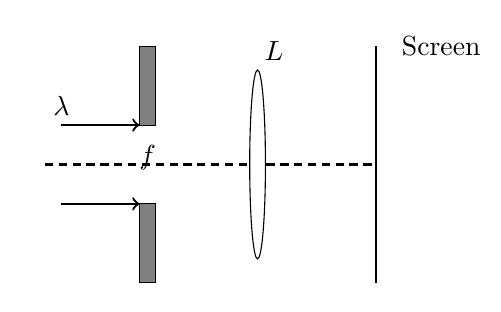
\begin{tikzpicture}
    \filldraw [fill=gray] (0,1.5) rectangle (0.2,0.5);
    \filldraw [fill=gray] (0,-1.5) rectangle (0.2,-0.5);
    \draw [thick,densely dashed] (-1.2,0)--(3,0);
    \draw [thick] (3,1.5)--(3,-1.5);
    \filldraw [fill=white] (1.5,0) ellipse (0.1 and 1.2);
    \foreach \y in {0.5,-0.5}
    \draw [thick,->,yshift=\y cm] (-1,0)--(0,0);
    \length{(1.5,-1.4)}{(3,-1.4)}{$f$}{(0.25,0)}
    \node [anchor=south] at (-1.2,0.5) {$\lambda$};
    \node [anchor=south] at (1.5,1.2) {$L$};
    \node [anchor=west] at (3,1.5) {Screen};
\end{tikzpicture}
\vfill
\end{paracol}
\vspace{-.75em}
\begin{solution}*
    条纹间距只与波长、焦距、缝宽有关,入射光方向不变,所以条纹间距、位置不变. \sokka{C}
\end{solution}

\begin{choice}{A}[牛顿环]
    牛顿环干涉装置上平凸透镜在垂直于平板玻璃的方向上,逐渐向下平移(靠近玻璃板)时,反射光形成的干涉条纹的变化情况是
    \begin{tasks}(2)
        \task 环纹向边缘扩散,环数不变
        \task 环纹向边缘扩散,环数增加
        \task 环纹向中心靠拢,环数不变
        \task 环纹向中心靠拢,环数增加
    \end{tasks}
\end{choice}
\begin{solution}*
    对于某条环,其光程差是确定的,所以环数不变;向边缘扩散光程差增大,可抵消透镜下移时导致的光程差减小.\sokka{A}
\end{solution}

\begin{choice}{B}[最大分辨力]
    假设用FAST装置探测波长为$20\mathrm{cm}$的宇宙射电信号,FAST望远镜的镜面直径为$500\mathrm{m}$,则装置的最小分辨角为
\begin{tasks}(4)
    \task $9.76\ee{-4}$
    \task $4.88\ee{-4}$
    \task $2.44\ee{-4}$
    \task $4.00\ee{-4}$
\end{tasks}
\end{choice}
\begin{solution}*
    $\theta=\frac{1.22\lambda}{D}=4.88\ee{-4}\mathrm{rad}$.\sokka{B}
\end{solution}

\vskip-2ex
\begin{paracol}{2}
    \begin{choice}{B}[双缝干涉]
        在双缝干涉实验中,屏幕$E$上的$P$点是明纹.若将缝$S_2$盖住,并在$S_1S_2$连线的垂直平分面处放一高折射率反射面$M$,如图所示.则此时$P$点
    \begin{tasks}(2)
        \task $P$点仍为明条纹
        \task $P$点为暗条纹
        \task 不能确定$P$点是明纹还是暗纹
        \task 无干涉条纹
    \end{tasks}   
    \end{choice}
    \switchcolumn\centering
    \vfill
    \begin{tikzpicture}[decoration={markings,mark=between positions .2 and .8 step 18mm with {\arrow{stealth}}}]
        \draw [very thick] (0,1.5)--(0,-1.5);
        \draw [thick,postaction=decorate] (-1,0)--(0,0.5)--(2,0.8);
        \draw [thick] (0,0.5)--(0.8,0);
        \draw [thick,postaction=decorate] (-1,0)--(0,-0.5)--(2,0.8);
        \draw [very thick] (0,0)--(1.8,0);
        \draw [very thick] (2,1.8)--(2,-1.8);
        \fill [pattern=north west lines] (0,0) rectangle (1.8,-0.2);
        \fill [pattern=north east lines] (2,1.8) rectangle (2.2,-1.8);
        \node [anchor=east] at (-1,0) {$S$} node [anchor=south east] at (0,0.5) {$S_1$} node [anchor=north east] at (0,-0.5) {$S_2$};
        \node [anchor=north] at (0.8,-0.2) {$M$} node [anchor=west] at (2.2,0.8) {$P$} node [anchor=north] at (2.1,-1.8) {$E$};
        \node at (-1,0) {$\times$};
    \end{tikzpicture}
    \vfill
\end{paracol}
\vspace{-.75em}
\begin{solution}*
    $S_1MP$、$S_2MP$长度相等,但平面镜使在反射中一条光路发生半波损失,两条光路的相位差变化$\pi$,所以$P$点由原来的明纹变为暗纹.\sokka{B}
\end{solution}

\begin{choice}{A}[迈克尔逊干涉仪]
    如果使迈克尔逊干涉仪的动镜移动$0.233\mathrm{mm}$,观察到$792$个条纹的移动,则所用照明单色光源的波长是多少?
\begin{tasks}(4)
    \task $588\mathrm{nm}$
    \task $294\mathrm{nm}$
    \task $442\mathrm{nm}$
    \task $552\mathrm{nm}$
\end{tasks}
\end{choice}
\begin{solution}*
    移动带来的光程差满足$\delta=2d=N\lambda$,由此得$\lambda=\frac{2d}{N}=588.38\mathrm{mm}$.\sokka{A}
\end{solution}

\begin{choice}{B}[光栅]
    某元素的特征光谱中含有波长分别为$\lambda_1=450\mathrm{nm},\ \lambda_2=750\mathrm{nm}$的谱线,在光栅光谱中这两种波长的谱线有重合现象,重叠处$\lambda_2$的谱线级数将是
\begin{tasks}(4)
    \task $2,\ 4,\ 6,\ 8,\cdots$
    \task $3,\ 6,\ 9,\ 12,\cdots$
    \task $4,\ 8,\ 12,\ 16,\cdots$
    \task $5,\ 10,\ 15,\ 20,\cdots$
\end{tasks}
\end{choice}
\begin{solution}*
    由光栅方程$d\sin\theta=k_1\lambda_1=k_2\lambda_2$得$k_2=\frac{k_1\lambda_1}{\lambda_2}$,取整值得$k_2=3,6,9,12,\cdots$.
\end{solution}

\section{填空题(共18分)}
\begin{problem}[弹簧振子][3]
    当弹簧振子以频率$f$做简谐振动时,它的动能的变化频率为\ans{$2f$}.
\end{problem}
\begin{solution}*
    动能和势能变化趋势相反,所以二者变化频率相同. 势能$E_p\propto x^2$,由于$x$是周期为$T$的余弦函数,所以$x^2$的周期为$\frac T2$,即势能的变化频率等于动能的变化频率等于$2f$.
\end{solution}

\begin{problem}[驻波][3]
    在均匀介质中,一列余弦波沿$Ox$轴传播,波动方程为$y_1=A\cos\ab(2\pi t+\frac{2\pi x}3)$ (SI),在$x=1\mathrm{m}$处反射,反射点为固定端,则反射波和入射波产生的驻波表达式为\ans{$2A\cos{\ab(2\pi t+\frac{7\pi}6)}\cos{\ab(\frac{2\pi x}{3}-\frac{7\pi}{6})}$}.
\end{problem}
\begin{solution}
\begin{itemize}
    \item 考虑反射带来的半波损失,$x=1\mathrm{m}$处反射波的振动方程为$y_{10}=A\cos\ab(2\pi t+\frac{2\pi}{3}+\pi)$.
    \item 反射后传播方向改变,考虑以$x=1$处为参考点需坐标变换$x'=x-1$,所以反射波的表达式为
    \[y_2=A\cos\ab(2\pi t+\frac{2\pi}{3}-\frac{2\pi(x-1)}3+\pi)=A\cos\ab(2\pi t-\frac{2\pi x}{3}+\frac{7\pi}3)\]
    \item 驻波表达式$y=y_1+y_2=2A\cos{\ab(2\pi t+\frac{7\pi}6)}\cos{\ab(\frac{2\pi x}{3}-\frac{7\pi}{6})}$.
\end{itemize}
\end{solution}

\begin{problem}[双缝干涉][6]
    如图所示,在双缝干涉实验中,若把一厚度为$e$、折射率为$n$的薄云母片覆盖在$S_1$缝上,中央明条纹将向\ans{上}移动;覆盖云母片后,两束相干光至原中央明纹$O$处的光程差为\ans{$(n-1)e$}.
\end{problem}
\begin{solution}*
    覆盖云母片后,通过$S_1$的光路光程差变大,为抵消这一变化中央明纹需上移使通过$S_2$的光路变长;原光程差为零,现光程差即云母片带来的光程差$\delta=ne-e=(n-1)e$.
\end{solution}

\begin{problem}[牛顿环][3]
    若把牛顿环装置(都是用折射率为$1.52$的玻璃制成的)由空气搬入折射率为$1.33$的水中,则干涉条纹\ans{变密}(变疏/变密).
\end{problem}
\begin{solution}*
    放入水中后每条条纹的光程差变大,为抵消这一变化条纹需向中心收缩,所以干涉条纹变密.
\end{solution}

\begin{problem}[弗琅禾费衍射][3]
    在单缝夫琅禾费衍射实验中,波长为$\lambda$的单色光垂直入射在宽度为$a=6\lambda$的单缝上,对应于衍射角为$30^\circ$的方向,单缝处波阵面可分成的半波带数目为\ans{6}.
\end{problem}
\begin{solution}*
    由衍射公式$a\sin{\theta}=k\lambda$得$k=3$,可分成的半波带数目为$2k=6$.
\end{solution}

\section{计算题(共46分)}
\begin{paracol}{2}
\begin{problem}[平面简谐波的波函数][10]
    一列平面简谐波在媒质中以波速$u=5\mathrm{m/s}$沿$x$轴正向传播,原点$O$处质元的振动曲线如图所示.
\begin{enumerate}
    \item 求解$x=25\mathrm{m}$处质元的振动方程并画出该点振动曲线.
    \item 求解波动方程,并画出$t=3\mathrm{s}$时的波形曲线.
\end{enumerate}
\end{problem}
\switchcolumn\centering
    \vfill
    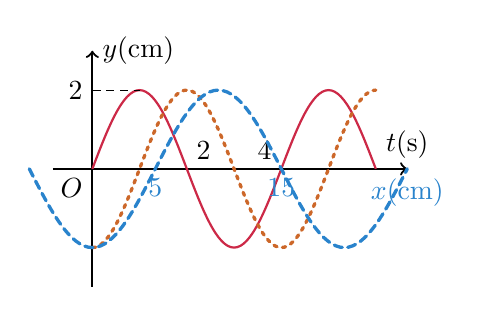
\begin{tikzpicture}
        \draw [->,thick] (-0.5,0)--(4,0) node [anchor=south] {$t(\mathrm{s})$} node [anchor=north] {\textcolor{H6}{$x(\mathrm{cm})$}};
        \draw [->,thick] (0,-1.5)--(0,1.5) node [anchor=west] {$y(\mathrm{cm})$};
        \draw[thick,H1] (0,0) sin (0.6,1) cos (1.2,0) sin (1.8,-1) cos (2.4,0) sin (3.0,1) cos (3.6,0);
        \draw [densely dashed] (0,1)--(.6,1) node [anchor=east,at start] {$2$};
        \node [anchor=north east] at (0,0) {$O$} node [anchor=south west] at (1.2,0) {$2$}  node [anchor=south east] at (2.4,0) {$4$};
        \draw [very thick,H2,dotted,line cap=round] (0,-1) cos (0.6,0) sin (1.2,1) cos (1.8,0) sin (2.4,-1) cos (3,0) sin (3.6,1);
        \draw [very thick,H6,densely dashed,line cap=round] (-.8,0) sin (0,-1) cos (.8,0) sin (1.6,1) cos (2.4,0) sin (3.2,-1) cos (4,0);
        \node [anchor=north] at (.8,0) {\textcolor{H6}{5}}  node [anchor=north] at (2.4,0) {\textcolor{H6}{15}};
    \end{tikzpicture}
    \vfill
\end{paracol}
\vspace{-.75em}
\begin{solution}
    \begin{enumerate}
        \item 由图知振幅$A=0.02\mathrm{m}$,角频率$\omega=\frac{2\pi}{T}=0.5\pi\mathrm{s}$. $t=0$时,$y=0,\ v>0$,初相$\varphi=-\frac\pi2$. 波动方程为\point{2}
        \[y=0.02\cos{\ab[\frac\pi2\ab(t-\frac{x}{5})-\frac\pi2]}\eqno\point{2}\]
        $x=25\mathrm{m}$处质元的振动方程为$y(x_0,t)=0.02\cos\ab(\frac\pi2t-\pi)$.\point{2}
        \item 波动方程见上问. $t=3\mathrm{s}$时的波形方程为
        \[y(x,t_0)=0.02\cos\ab(-\frac{\pi}{10}x+\pi)\eqno\point{2}\]
    \end{enumerate}
\end{solution}

\vskip-2ex
\begin{paracol}{2}
\begin{problem}[光程和光程差][8]\footnote{\kaishu 选自37th CPhO预赛试题第10题,原题未并提供参考图片.}
    一艘船(如图中$S$)在$25\mathrm{m}$高的桅杆($SS'$)上装有一天线(如图中$S''$),不断发射某种波长的无线电波,已知波长在$2-4\mathrm{m}$范围内,在高出海平面$150\mathrm{m}$的悬崖顶($OP$)上有一接收站$P$能收到这无线电波,但当那艘船驶至离悬崖底部$OS=2\mathrm{km}$时,接收站就收不到无线电波.设海平面完全反射这无线电波,求所用无线电波的波长.
\end{problem}
\switchcolumn\centering
\vfill
\begin{tikzpicture}[scale=0.8]
    \coordinate [label=below left:{$S$}] (S) at (0,0);
    \coordinate [label=above left:{$S'$}] (S') at (0,1);
    \coordinate [label=below left:{$S''$}] (S'') at (0,-1);
    \coordinate [label=below:{$M$}] (M) at (1.5,0);
    \coordinate [label=above:{$P$}] (P) at (6,3);
    \coordinate [label=below:{$O$}] (O) at (6,0);
    \draw [thick,line join=round,line cap=round] (P) -- (O) -- (S) -- (S');
    \draw [thick,dashed,line join=round] (P) -- (S) -- (S'') -- (M);
    \draw [very thick,line cap=round,densely dashed,H1] (S') -- (P);
    \draw [very thick,line cap=round,dotted,H1] (S') -- (M) --  (P);
    \length{(-.25,0)}{(-.25,1)}{$a$}{(0,0.25)}
    \pic ["$\theta$", draw, thick, angle radius=5mm, angle eccentricity=1.5] {angle=O--S--P};
    \pic ["$\theta'$", draw, thick, angle radius=5mm, angle eccentricity=1.5] {angle=O--M--P};
    \pic ["$\Delta\theta$", draw, thick, angle radius=10mm, angle eccentricity=1.5] {angle=S--P--M};
    \draw [thick] (S') -- (0.75,-0.5) coordinate [label=below:$K$] (foot);
    \pic ["$\theta$", draw, thick, angle radius=3mm, angle eccentricity=2] {angle=S''--S'--foot};
    \length{($(S'')+({0.5*sin(atan(2/3))},{-0.5*cos(atan(2/3))})$)}{($(foot)+({0.5*sin(atan(2/3))},{-0.5*cos(atan(2/3))})$)}{$\scriptstyle 2a\sin\theta$}{({0.5*cos(atan(2/3))},{0.5*sin(atan(2/3))})}
    \length{($(S)-(0,2)$)}{($(O)-(0,2)$)}{$2\mathrm{km}$}{(1.5,0)}
    \length{($(O)+(0.5,0)$)}{($(P)+(0.5,0)$)}{$150\mathrm{m}$}{(0,0.5)}
    \draw [dashed,H4] (S') --++ (6,0) -- (P);
    \draw [dashed,H6] (S'') --++ (6,0) -- (P);
\end{tikzpicture}
\vfill
\end{paracol}
\vspace{-.75em}
\begin{solution}
    考虑半波损失,经海平面反射的光波与直达$P$点的光波之间的光程差为
    \[\delta=2a\sin\theta+\frac\lambda2\eqno\point{3}\]
    由几何关系$\sin\theta=\sin\arctan\ab(\frac{150}{2000})=0.075$. 利用干涉相消条件得无线电波长为\point{2}
    \[\delta=\frac{2k+1}{2}\lambda,\ \lambda=\frac{2a\sin\theta}{k}\xlongequal[2<\lambda<4]{k=1}3.74\mathrm{m}\eqno\point{3}\]
    \textbf{本题中$\Delta\theta$不可忽略,不得认为$\theta=\angle PMO$! 否则会得到$k=2.18$.}
    \vskip1ex\hrule\vskip1ex
    另一种更精确的解法是直接计算两条光路的长度之差\footnote{值得一提的是,因上一种解法近似认为$S'K\bot S''K$,相对于这种解法有$7.73\ee{-3}\%$的误差(小数点第四位及以后不同).}
    \[\begin{aligned}
        \delta&=\overline{S''P}-\overline{S'P}+\frac\lambda2=\sqrt{\ab(\overline{SO})^2+\ab(\overline{OP}+\overline{SS''})^2}-\sqrt{\ab(\overline{SO})^2+\ab(\overline{OP}-\overline{SS''})^2}+\frac\lambda2\\
        &=\sqrt{2000^2+(150+25)^2}-\sqrt{2000^2+(150-25)^2}+\frac\lambda2=\frac{2k+1}{2}\lambda
    \end{aligned}\]

    解得$\lambda\xlongequal{k=1}3.74\mathrm{m}$.
\end{solution}

\begin{problem}[薄膜干涉][10]
波长为$\lambda=500\mathrm{nm}$的单色光垂直入射到\textbf{置于空气中}的上下表面平行的薄膜上,已知膜的折射率$n=1.25$,求反射光、透射光最强时膜的最小厚度.
\end{problem}
\begin{solution}*
    两个表面反射光光程差为$\delta=2ne+\frac\lambda2$. 分别由反射光干涉相长$\delta=k\lambda$和相消$\delta=\frac{2k+1}{2}\lambda$得\point{4}
    \[e_{\min_1}=\frac{\lambda}{4n}=100\mathrm{nm},\ e_{\min_2}=\frac{\lambda}{2n}=200\mathrm{nm}\eqno\point{4}\]
\begin{itemize}
    \item 反射光干涉相长时,反射光最强,膜的最小厚度为$e_{\min_1}=100\mathrm{nm}$.\point{1}
    \item 反射光干涉相消时,透射光最强,膜的最小厚度为$e_{\min_2}=200\mathrm{nm}$.\point{1}
\end{itemize}
\end{solution}

\vskip-2ex
\begin{paracol}{2}
\begin{problem}[光栅][12]
    如右图所示,$AB$之间的虚线为一透射式光栅,该光栅在$1\mathrm{mm}$内刻画有$500$条狭缝,单条狭缝的缝宽为$a=0.5\mu\mathrm{m}$,一波长为$\lambda=500\mathrm{nm}$的单色平行光斜入射在该光栅上,入射角$\theta=30^\circ$(从光栅光轴下方入射),在光栅后放置凸透镜和观察屏(屏位于透镜的焦平面处),问屏上能看到哪几级谱线?
\end{problem}
\switchcolumn\centering
\vfill
\begin{tikzpicture}[decoration={markings,mark=between positions .25 and .8 step 20mm with {\arrow{stealth}}}]
    \filldraw [thick,fill=gray] (0,1.6) rectangle (0.15,0.5);
    \draw [densely dashed,thick] (0,0.5)--(0,-0.5);
    \filldraw [thick,fill=gray] (0,-1.6) rectangle (0.15,-0.5);
    \draw [densely dashed,thick] (-1.5,0)--(2,0);
    \coordinate (b) at (-1.5,0);
    \coordinate (a) at (0,0);
    \coordinate (c) at (-1,-0.4);
    \coordinate (d) at (1.5,0.2);
    \coordinate (e) at (2,0);
    \foreach \a in {-0.5,-0.25,0,0.25,0.5}
    \draw [yshift=\a cm,thick,postaction=decorate,->] (-1,-0.4)--(0,0)--(1.5,0.2);
    \pic["$\theta$", draw=black, very thick, angle
    eccentricity=1.35, angle radius=24]{angle=b--a--c};
    \pic["$\varphi$", draw=black, very thick, angle
    eccentricity=1.35, angle radius=36]{angle=e--a--d};
    \node[anchor=east] at (0,0.6) {$A$} node[anchor=east] at (0,-0.6) {$B$};
\end{tikzpicture}
\vfill
\end{paracol}
\vspace{-.75em}
\begin{solution}*
    光栅常数$d=\frac{1\ee{-3}}{500}=2\mu\mathrm{m}$. 由于光栅方程\point{2}
    \[d(\sin\varphi-\sin\theta)=k\lambda\eqno\point{2}\]
\begin{itemize}
    \item 令$\varphi=\pm 90^\circ$得$k_{\min}=-6,\ k_{\max}=2$. 由缺级条件得$k'=\frac{d}{a}=\pm 4$,第$-4$级缺级.\point{4}
    \item 由于$\varphi$无法取到$\pm 90^\circ$,所以屏上可见主极大级次为$k=0,\ \pm 1,\ -2,\ -3,\ -5$.\point{4}
\end{itemize}
\end{solution}

\begin{problem}[驻波][6]
    由振动频率为$400\mathrm{Hz}$的音叉在两端固定拉紧的弦线上建立驻波.这个驻波共有三个波腹,其振幅为$0.30\mathrm{cm}$,波在弦上的速度为$320\mathrm{m/s}$.
\begin{enumerate}
    \item 求此弦线的长度.
    \item 若以弦的中点为坐标原点,试写出弦线上驻波的表达式.
\end{enumerate}
\end{problem}
\begin{solution}
\begin{enumerate}
    \item 由题意得弦长为$1.5$个波长,即$l=1.5\lambda=1.5\frac{u}{f}=1.2\mathrm{m}$.\point{2}
    \item 驻波的角频率$\omega=2\pi f=800\pi$,波矢$k=\frac{2\pi}{\lambda}=\frac{5}{2}\pi$. 设驻波的表达式为
    \[y=3\ee{-3}\cos\ab(800\pi t+\phi)\cos\ab(\frac52\pi x+\varphi)\eqno\point{2}\]
    中点$x=0$处是波腹,所以$\cos\varphi=1,\ \varphi=0\ \text{or}\ \pi$. 所以驻波的表达式为
    \[y=\pm 3\ee{-3}\cos\ab(800\pi t+\phi)\cos\ab(\frac52\pi x)\eqno\point{2}\]
    符号$\pm$对应$\varphi$的两个解,$\phi$由初始条件决定.
\end{enumerate}
\end{solution}
\end{document}